
\begin{figure}[!t]
    \centering
	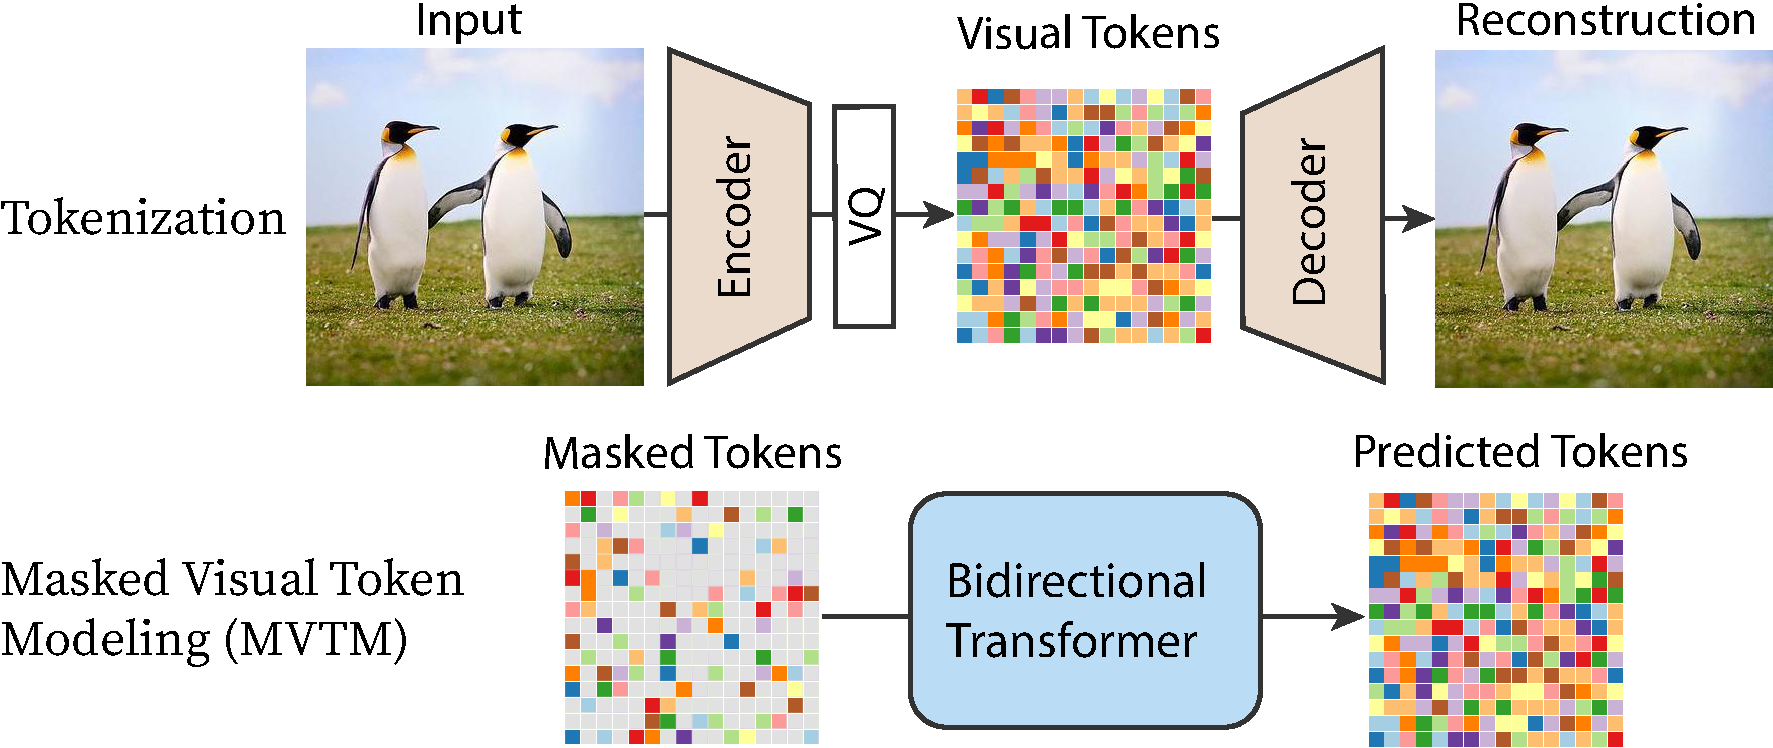
\includegraphics[width=\linewidth]{figures/pipeline_figure.pdf}
    % \vspace{-25mm}
    \caption{\textbf{Pipeline Overview.} \model follows a two-stage design, with 1) a tokenizer that tokenizes images into visual tokens, and 2) a bidirectional tranformer model that performs MVTM, i.e. learns to predict visual tokens masked at random.}
    \vspace{-3mm}
    \label{fig:pipeline}
\end{figure}
\section{Method}
\label{sec:method}
Our goal is to design a new image synthesis paradigm utilizing parallel decoding and bi-directional generation.

We follow the two-stage recipe discussed in \ref{sec:related_synthesis}, as illustrated in Figure~\ref{fig:pipeline}. Since our goal is to improve the second stage, we employ the same setup for the first stage as in the VQGAN model~\cite{Esser21vqgan}, and leave potential improvements to the tokenization step to future work.

For the second stage, we propose to learn a bidirectional transformer by \textit{Masked Visual Token Modeling} (MVTM). We introduce MVTM training in \ref{ssec:model} and the sampling procedure in \ref{ssec:decoding}. We then discuss the key technique of masking design in \ref{ssec:masking}. 


\subsection{MVTM in Training}
\label{ssec:model}
\newcommand{\unknownmask}[0]{{\mathbf{M}}}
\newcommand{\mathy}[0]{{\mathbf{Y}}}
\newcommand{\knownmask}[0]{{\overline{\mathbf{M}}}}
Let $\mathy=[y_i]_{i=1}^N$ denote the latent tokens obtained by inputting the image to the VQ-encoder, where $N$ is the length of the reshaped token matrix, and $\unknownmask=[m_i]_{i=1}^N$ the corresponding binary mask. During training, we sample a subset of tokens and replace them with a special \texttt{[MASK]} token. The token $y_i$ is replaced with \texttt{[MASK]} if $m_i=1$, otherwise, when $m_i=0$, $y_i$ will be left intact. 

The sampling procedure is parameterized by a mask scheduling function $\gamma (r) \in (0,1]$, and executes as follows: we first sample a ratio from $0$ to $1$, then uniformly select $\lceil \gamma(r) \cdot N \rceil$ tokens in $\mathy$ to place masks, where $N$ is the length. The mask scheduling significantly affects the quality of image generation and will be discussed in \ref{ssec:masking}.

Denote $Y_{\knownmask}$ the result after applying mask $\unknownmask$ to $\mathy$.
The training objective is to minimize the negative log-likelihood of the masked tokens:
\begin{equation}
\label{eq:loss}
\mathcal{L}_{\text{mask}} = - \mathop{\mathbb{E}} \limits_{\mathy  \in \mathcal{D}} \Big[ \sum_{\forall i \in [1,N], m_i=1} \log p(y_i| Y_{\knownmask}) \Big],
\end{equation}

\noindent Concretely, we feed the masked $Y_{\knownmask}$ into a multi-layer bidirectional transformer to predict the probabilities $P(y_i | Y_{\knownmask} )$ for each masked token, where the negative log-likelihood is computed as the cross-entropy between the ground-truth one-hot token and predicted token.
Notice the key difference to autoregressive modeling: the conditional dependency in MVTM has two directions, which allows image generation to utilize richer contexts by attending to all tokens in the image.

\subsection{Iterative Decoding}
\label{ssec:decoding}
In autoregressive decoding, tokens are generated sequentially based on previously generated output. This process is not parallelizable and thus very slow for image because the image token length, \eg 256 or 1024, is typically much larger than that of language. We introduce a novel decoding method where all tokens in the image are generated simultaneously in parallel. This is feasible due to the bi-directional self-attention of MTVM. 

In theory, our model is able to infer all tokens and generate the entire image in a single pass. We find this challenging due to inconsistency with the training task. Below, the proposed iterative decoding is introduced.
To generate an image at inference time, we start from a blank canvas with all the tokens masked out, \ie $Y_\unknownmask^{(0)}$. For iteration $t$, our algorithm runs as follows: 
 
 \vspace{-2mm}
 \begin{enumerate}
     \item \textbf{Predict.}  Given the masked tokens $Y_\unknownmask^{(t)}$ at the current iteration, our model predicts the probabilities, denoted as $p^{(t)} \in \mathbb{R}^{N \times K}$, for all the masked locations in parallel.  \\ \vspace{-5mm}
     \item \textbf{Sample.} At each masked location $i$, we sample a token $y_i^{(t)}$ based on its prediction probabilities $p_i^{(t)} \in \mathbb{R}^K$ over all possible tokens in the codebook. After a token $y_i^{(t)}$ is sampled, its corresponding prediction score is used as a ``confidence" score indicating the model's belief of this prediction. 
     For the unmasked position in $Y_\unknownmask^{(t)}$, we simply set its confidence score to $1.0$. \\ \vspace{-5mm}
    \item \textbf{Mask Schedule.} We compute the number of tokens to mask according to the mask scheduling function $\gamma$ by $n = \lceil \gamma(\frac{t}{T}) N \rceil$, where $N$ is the input length and $T$ is the total number of iterations.
    \item \textbf{Mask.} We obtain $Y_\unknownmask^{(t+1)}$ by masking $n$ tokens in $Y_\unknownmask^{(t)}$. The mask $\unknownmask^{(t+1)}$ for iteration $t+1$ is calculated from:\vspace{-2mm}
        \begin{equation*}
         m_{i}^{(t+1)} = 
        \begin{cases}
            1,  & \text{if $c_i < {\text{sorted}}_j(c_j)[n]$.}\\
            0,  & \text{otherwise.}\vspace{-2mm}
        \end{cases},
        \end{equation*}
    where $c_i$ is the confidence score for the $i$-th token.

 \end{enumerate}


The decoding algorithm synthesizes an image in $T$ steps. At each iteration, the model predicts all tokens simultaneously but only keeps the most confident ones. The remaining tokens are masked out and re-predicted in the next iteration. The mask ratio is made decreasing until all tokens are generated within $T$ iterations. In practice, the masking tokens are randomly sampled with temperature annealing to encourage more diversity, and we will discuss its effect in \ref{ssec:ablation}. Figure~\ref{fig:decoding} illustrates an example of our decoding process. It generates an image in $T=8$ iterations, where the unmasked tokens at each iteration are highlighted in the grid, \eg when $t=1$ we only keep 1 token and mask out the rest.

\subsection{Masking Design}
\label{ssec:masking}

We find that the quality of image generation is significantly affected by the masking design. We model the masking procedure by a mask scheduling function $\gamma (\cdot)$ that computes the mask ratio for the given latent tokens. As discussed, the function $\gamma$ is used in both training and inference. During inference time, it takes the input of $0/T, 1/T, \cdots, (T-1)/T$ indicating the progress in decoding. In training, we randomly sample a ratio $r$ in $[0,1)$ to simulate the various decoding scenarios.

BERT uses a fixed mask ratio of 15\%~\cite{Devlin19bert}, \ie, it always masks 15\% of the tokens, which is unsuitable for our task since our decoder needs to generate images from scratch. New masking scheduling is thus needed. Before discussing specific schemes, we first examine the property of the mask scheduling function. First, $\gamma(r)$ needs to be a continuous function bounded between $0$ and $1$ for $r \in [0,1]$. Second, $\gamma(r)$ should be (monotonically) decreasing with respect to $r$, and it holds that $\gamma(0)\rightarrow1$ and $\gamma(1)\rightarrow0$. 
The second property ensures the convergence of our decoding algorithm.


This paper considers common functions and makes simple transformations so that they satisfy the properties. Figure~\ref{fig:scheduling} visualizes these functions which are divided into three groups:
\begin{itemize}
    \vspace{-2mm}
    \item \textbf{Linear function} is a straightforward solution, which masks an equal amount of tokens each time.
    \vspace{-2mm}
    \item \textbf{Concave function} captures the intuition that image generation follows a less-to-more information flow. In the beginning, most tokens are masked so the model only needs to make a few correct predictions for which the model feel confident. Towards the end, the mask ratio sharply drops, forcing the model to make a lot more correct predictions. The effective information is increasing in this process. The concave family includes cosine, square, cubic, and exponential.
    \vspace{-2mm}
    \item \textbf{Convex function}, conversely, implements a more-to-less process. The model needs to finalize a vast majority of tokens within the first couple of iterations. This family includes square root and logarithmic.
    
    \vspace{-2mm}
\end{itemize}

We empirically compare the above mask scheduling functions in \ref{ssec:ablation} and find the $\text{cosine}$ function works the best in all of our experiments.